 \documentclass{llncs}

\usepackage{pslatex}
\usepackage{url}
\usepackage{latexsym}
\usepackage{alltt,verbatim,graphicx}
\usepackage{amsmath,amssymb,url}

\usepackage{AMMALanguages}

%\newcommand{\ecal}{\mathcal{E}}
\newcommand{\rcal}{\mathcal{R}}
\newcommand{\tcal}{\mathcal{T}}
\newcommand{\rews}{\rightarrow}
\newenvironment{code2}{\begin{verbatim}}{\end{verbatim}}

\newcommand{\ignore}[1]{}
\newcommand{\tcode}[1]{\text{\tt #1}}
\newcommand{\obj}[1]{\langle \tcode{#1} \rangle}

\newcommand{\paco}[1]{\textcolor{red}{[Paco writes: #1]}}
\newcommand{\camilo}[1]{\textcolor{blue}{[Camilo writes: #1]}}


\title{Tool Interoperability in the
Maude Formal Environment}

\author{Francisco Dur\'an\inst{1} \and Camilo Rocha\inst{2} \and Jos\'e M. \'Alvarez\inst{1}}

\institute{
Universidad de M\'alaga, Spain. %\email{duran@lcc.uma.es} 
\and
University of Illinois at Urbana-Champaign, IL, USA. %\email{meseguer@uiuc.edu}
}

%
% Margin notes
%
\newcounter{marginalnote}
\setcounter{marginalnote}{1}
\renewcommand{\themarginalnote}{\arabic{marginalnote}}
	
\setlength{\marginparwidth}{3cm}
	
\newcommand{\mnote}[1]
{\raisebox{1ex}{\scriptsize (\themarginalnote)}%
\marginpar{\footnotesize\raggedright\indent
\raisebox{1ex}{\scriptsize (\themarginalnote)} %\textcolor{red}
                                               {#1}}%
\addtocounter{marginalnote}{1}}
%
\newcommand{\rcal}{\mathcal{R}}
\newcommand{\ignore}[1]{}

\begin{document}

\maketitle

\begin{abstract}
We present the Maude Formal Environment (MFE), 
an executable formal specification in Maude within which a 
user can seamlessly interact with the Maude Termination Tool,
the Maude Sufficient Completeness Checker, the Church-Rosser
Checker, the Coherence Checker, and the Maude Inductive
Theorem Prover.
We explain the high-level design decisions behind MFE,
give a summarized account of its main features, and
illustrate with an example the interoperation of
the tools available in its current release.
\end{abstract}

\section{Introduction}

%There is a great deal of interest today in developing
%multipurpose environments that combine declarative
%programming with specification languages and useful
%formal analysis tools (see, e.g., \cite{Mossakowski-Maeder-Luttich:2007,Franssen-Brand:2009,Hemer-Long-Strooper:2005,uitp-web-page,Aspinall-Luth:2007}).
Maude~\cite{CDELMMT:2007-book} is a reflective declarative 
language and system based on rewriting logic in which computation
corresponds to efficient deduction by rewriting.
%As part of the Maude distribution or as an extension,
Several tools for the formal analysis of Maude modules
have been available for a number of years. They include
an inductive theorem prover~\cite{Clavel-Palomino-Riesco:2006}
for equational specifications,
and an LTL model checker~\cite{Eker-Meseguer-Sridharanarayanan:02},
a reachability analysis tool~\cite{CDELMMT:2007-book},
and an invariant analyzer~\cite{Rocha-Meseguer:2011-tr}
for rewrite specifications.
However, many verification techniques such as the ones
implemented by the tools just mentioned assume that the input
module satisfies certain properties. For example, any verification
task with the LTL model checker on a rewrite specification 
$\rcal = (\Sigma,E\cup A,R)$ assumes that $\rcal$ satisfies the
so-called {\em executability requirements}, namely, that
the equations $E$ specifying the functional part 
of $\rcal$ are both ground terminating and ground
Church-Rosser modulo the structural axioms $A$, and
that the rules $R$ specifying the concurrent transitions
of $\rcal$ are ground coherent w.r.t. $E$ modulo $A$.
If they do not hold, 
then any analysis performed by the LTL model checker on $\rcal$
can in general lead to unsound and incomplete results.

\ignore{
, several tools have been available for a number of years, such as an LTL model checker~\cite{Eker-Meseguer-Sridharanarayanan:02,CDELMMT:2007-book}, a reachability analysis tool~\cite{CDELMMT:2007-book}, an inductive theorem prover~\cite{Clavel-Palomino-Riesco:2006}, or an invariant analyzer~\cite{Rocha-Meseguer:2011-tr}.
%We may use these tools, e.g., to prove inductive theorems about an 
%equational theory $(\Sigma,E \cup A)$, or to model check temporal logic 
%properties for a rewrite theory $\mathcal{R} = (\Sigma,E \cup A,R,\phi)$. 
However, many verification methods, including the ones just mentioned,
rely on specific properties.
Even before any formal verification is attempted, the (ground) Church-Rosser property of an equational theory $(\Sigma,E \cup A)$ and the (ground) coherence of a rewrite theory $\mathcal{R} = (\Sigma,E \cup A,R,\phi)$ are essential \emph{executability requirements}, without which the execution of $(\Sigma,E \cup A)$ as a functional program (resp., of $\mathcal{R} = (\Sigma,E \cup A,R,\phi)$ as a concurrent program) may yield unpredictable results.

Thus, properties such as (ground) Church-Rosser, (ground) coherence, (operational) termination, and sufficient completeness, and methods to check them, are essential, both for executability purposes and as a basis for verifying many other properties, such as, for example, proving inductive theorems of a functional program, or correct model checking of temporal logic properties for a concurrent program.}

Maude has been successfully used as a {\em metatool}
in the creation of tools for verifying properties of its modules~\cite{clavel99}.
In this sense, previous work presented in~\cite{CDHLMO:2007}
describes the main features of several tools concerned with 
the analysis of either Maude modules
or of extensions of Maude.
However, these tools work in isolation, 
making it inconvenient to switch between their execution environments
and difficult to exchange data between them.
In response to these limitations, 
we present the Maude Formal Environment (MFE),
an executable and highly extensible software infrastructure
within which a user can interact with several 
tools to mechanically verify properties of Maude modules.
In MFE, tools can interoperate to discharge proof obligations
of different nature without switching between different
execution environments.
The integration of different tools inside 
MFE's common environment presents the user with a consistent user interface,
a mechanism to keep track of pending proof obligations,
and allows the execution of several instances of each tool,
among other features.

The following tools are currently available as part of MFE: the Maude Termination
Tool (MTT) can be used to prove termination of equational and rewrite specifications~\cite{Duran-Lucas-Meseguer:2008-ijcar}; %DLMMU:2008-hosc,
the Sufficient Completeness Checker (SCC)
can be used to check completeness and freeness of equational specifications, and deadlock freedom of rewrite specifications~\cite{Hendrix:2008,Rocha-Meseguer:2010}; %Hendrix-Meseguer-Ohsaki:2006
the Church-Rosser Checker (CRC) can be used to check
ground confluence and sort-decreasingness of equational
specifications~\cite{Duran-Meseguer:2010-wrla-crc}; %Duran-Meseguer:2011
the Coherence Checker (ChC) can be used to check
the ground coherence of rewrite specifications~\cite{Duran-Meseguer:2010-wrla-chc}; %,Duran-Meseguer:2011
and the Inductive Theorem Prover (ITP) can be used to verify inductive properties
of equational specifications~\cite{Clavel-Palomino-Riesco:2006,Hendrix:2008}. %Clavel-Palomino-Riesco:2006,

{\bf Outline.} In Section~\ref{sec.des} we give a high-level overview
of MFE's design features
% and in Section~\ref{sec.use} 
and we explain some of the
commands available. % from MFE. 
In Section~\ref{sec.case} we
illustrate MFE's main functionality
with a case study in which a user interacts with several of the tools in the environment.  
%the MTT, SCC, CRC, ChC, 
%and ITP in the task of verifying the mutual exclusion property for
%the Bakery Protocol.
%The MFE executable module in Maude
The executables, a white paper explaining MFE's design,
examples, and preliminary documentation, are available
at \url{http://maude.lcc.uma.es/MFE}. For further details on the tools
available in MFE please check the given references.

\section{MFE's Design and Main Features}
\label{sec.des}

%As it is the case with some of these tools and with
%some other ones~\cite{CDELMMT:2007-book}, 
MFE has been implemented as an extension of Full Maude~\cite{Duran-Meseguer:2007-scp}, %,Duran:1999-thesis
thus benefiting from its functionality and flexibility.  
Full Maude is an extension of Maude written in Maude itself that has become a common 
infrastructure on top of which tools can be built.
In MFE, for instance, tools provided by Maude such as
its LTL model checker and search command are available, as well as
modules defined in Full Maude (including object-oriented ones)
are directly amenable to formal verification.
%, and commands for loading
%modules, theories, and views are accessible.

MFE is highly extensible and amenable to tool interoperability
given its modular design and the fact that it imposes no constraint
on how each tool should model its particular domain or 
 maintains its internal state.
MFE is modeled in Maude as an interactive object-based system where 
tools are objects, the communication mechanism
is message passing, and user interaction is available through Full Maude.
Integration and interoperation of tools within MFE is module-centric,
given that its main purpose is to support formal analysis of Maude modules.

The object-oriented model of MFE consists of three classes: 
the class \texttt{Proof} of proof objects which keep the state of specific proof requests,
the class \texttt{Tool} of tool objects which manage proof objects, and
a class \texttt{Controller}
which inherits from the Full Maude's \texttt{DatabaseClass} 
and provides a centralized entry point for 
handling requests to the formal environment.

The \texttt{Controller} object defines the behavior of the 
environment and its tools with the user. 
The user interacts with the environment via commands
which are encapsulated as messages in the object configuration. Each
tool object and the controller object have a module defining 
the signature of the commands it can handle. 
The controller handles any command it can parse;
since this object extends Full Maude, it handles its own commands
and Full Maude ones.
If the controller receives a command it cannot parse, then it
delegates the message to the {\em active} tool (previously selected by the user). 
If the active tool can parse the delegated command, 
then it notifies the controller and handles the command.
Otherwise, it will notify the failure to the controller,
which in turn will output an error message of the 
failed command to the user.

Classes \texttt{Proof} and \texttt{Tool} define some basic 
functionality that can be inherited by any new tool.
Class {\tt Tool}, for example, defines a set of attributes that
are convenient for supporting multiple instances of a tool and
predefines some rewrite rules for managing the life cycle of proof objects.
However, new tools can be added to MFE without inheriting from
any of these two classes. 

%\section{On the Use of MFE}
%\label{sec.use}

MFE provides the following user commands, in addition to the ones inherited from Full Maude:

\begin{description}
\item[\texttt{  \small(select tool <tool-name> .)}]
%\noindent \texttt{  \small(select tool <tool-name> .)} 
sets \texttt{\small<tool-name>} as the {\em active} tool.
\item[\texttt{  \small(MFE help .)}] 
%\noindent \texttt{  \small(MFE help .)}  
shows MFE's help information.
\item[\texttt{  \small(show global state .)}] 
%\noindent \texttt{  \small(show global state .)}  
shows the state of the environment.
\end{description}

Any command that cannot be parsed against MFE's grammar is delegated
to the active tool. In this way, user interaction with any
tools remains almost the same as before its integration in MFE.
We refer the reader to MFE's documentation and to each tool's documentation
for a detailed account of commands, restrictions, and additional examples. 

In order to be flexible,
MFE does not define any policy for naming tool commands.
However, as a general guideline for using the environment, 
it is recomended that the tools provide at least the following
commands, as it is the case with the tools available
in MFE's  current release:

\begin{description}
\item[\texttt{  \small(<tool-name> help .)}]
%\noindent \texttt{  \small(<tool-name> help .)}
shows the help information of tool \texttt{\small<tool-name>}.
%information on the commands available in the active tool.
\item[\texttt{  \small(show state .)}]
%\noindent \texttt{  \small(show state .)}
shows the state of the tool.
\end{description}

MFE's design supports non-trivial dependencies
among tools and potential interaction complexity.
For instance, a ground coherence check on a rewrite specification
assumes the ground termination and ground Church-Rosser properties
on its equational subspecification, and may produce a number of inductive
proof obligations that could be discharged with help of ITP.
Figure~\ref{fig.tool-dep} depicts the tool-dependency graph for
the current tools in MFE.

%\vspace{-0.6cm}

\begin{figure}%[htbp]
\begin{center}
%\fbox{
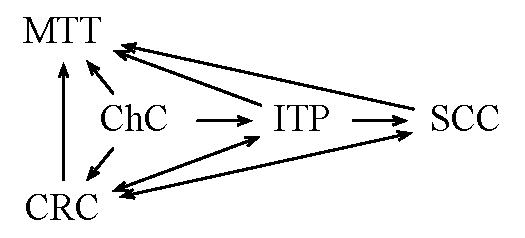
\includegraphics[width=6cm]{tool-dep}
%}
\caption{Tool-dependency graph in MFE.}
\label{fig.tool-dep}
\end{center}
\end{figure}

\vspace{-0.8cm}

A tool in MFE keeps track of both its pending and discharged proof obligations.
It can submit proof obligations to other tools by means of a {\tt submit} command
and then be notified when these are discharged. When all proof obligations
in the verification process of a module's property are discharged, the corresponding tool notifies 
the success result to the user or to the tool originating the verification task.

Of course, tools in general can impose constraints on its inputs. For instance, 
SCC does not support parametric modules but, nevertheless, proofs for such modules
could be obtained by hand or by using a different tool. MFE offers
a {\tt trust} command for keeping track of proofs obtained outside MFE.

Finally, for tools which depend on external
utilities not directly available from Maude such as MTT and SCC, 
we have extended the latest release of the Maude system
with {\em built-in} operators associated with appropriate
C++ code that interacts with the external tools.
A similar extension was previously performed for 
the SCC~\cite{Hendrix:2008}.

\section{Case Study: Ground Coherence of the Bakery Protocol}
\label{sec.case}

We explain how MFE can be used to prove the ground coherence of
module \verb"BAKERY", yet another Maude specification of the Bakery Protocol.
The Bakery Protocol is a classical solution by Lamport to the problem 
of achieving mutual exclusion between processes.
The protocol is based on the procedure commonly used in bakeries
where a customer is assigned a ticket number upon arrival.
Here, a process is a term with sort \verb"BProcess" built from operator
\verb"<_,_,_>" that takes a natural number with sort \verb"Nat"
as identifier, a constant term \verb"sleep", \verb"wait", or \verb"crit"
with sort \verb"Mode" as current state, and
a natural number as ticket number.
A term with sort \verb"BState" is a multiset of processes,
where each process is a singleton multiset and union is denoted by juxtaposition.
A term with sort \verb"GBState" represents the system's state
and it is built
from operator \verb"[[_]]" that takes a multiset of processes as argument.

The concurrent behavior of the Bakery Protocol is modeled 
in the \verb"BAKERY" system module as follows. %with the following rewrite rules.

\begin{lstlisting}[style=AMMA, language=Maude, numbers=none]
 (mod BAKERY is 
   protecting MNAT . 

   sorts Id Mode BProcess BState GBState .
   ops sleep wait crit : -> Mode [ctor] .
   op <_`,_`,_> : MNat Mode MNat -> BProcess [ctor] .
   subsort BProcess < BState .
   op __ : BState BState -> BState [ctor assoc comm id: none] .
   op none : -> BState [ctor] .
   op `[`[_`]`] : BState -> GBState [ctor] .

   var P : Mode . vars I N M : MNat . var BSt : BState .

   ---- max of the numbers assigned to processes (0 if none)
   op maxNumber : BState -> MNat .
   op maxNumber : BState MNat -> MNat .
   eq maxNumber(< I, P, N > BSt) = max(N, maxNumber(BSt)) .
   eq maxNumber(none) = 0 .

   ---- min. of the nonzero numbers assigned to processes (0 if none)
   op minNzNumber : BState -> MNat .
   op minNzNumber : BState MNat -> MNat .
   eq minNzNumber(< I, P, 0 > BSt) = minNzNumber(BSt) .
   eq minNzNumber(< I, P, s N > BSt) = minNzNumber(BSt, s N) .
   eq minNzNumber(none) = 0 .
   eq minNzNumber(< I, P, 0 > BSt, M) = minNzNumber(BSt, M) .
   eq minNzNumber(< I, P, s N > BSt, M) = minNzNumber(BSt, min(M, s N)) .
   eq minNzNumber(none, M) = M .

   rl [s2w] : [[ < I, sleep, 0 > BSt ]] 
     => [[ < I, wait, s maxNumber(BSt) > BSt ]] .
  crl [w2c] : [[ < I, wait, N > BSt ]] 
     => [[ < I, crit, N > BSt ]] 
     if N = minNzNumber(< I, wait, N > BSt) .
   rl [c2s] : [[ < I, crit, N > BSt ]] 
     => [[ < I, sleep, 0 > BSt ]] .
 endm)
\end{lstlisting}

Operators \verb"maxNumber" and \verb"minNzNumber" operate on terms
with sort \verb"BState" and compute, respectively, the maximum and
minimum ticket numbers in a multiset of processes, or \verb"0" if none.

In MFE, \verb"BAKERY"'s executability properties can be proved in
different order. For instance, we first activate CRC and use its
\verb"check Church-Rosser" command to first verify \verb"BAKERY"'s
equational subspecification Church-Rosser.

\begin{lstlisting}[style=AMMA, language=MaudeCommand, numbers=none]
 Maude> (select tool CRC .)
 The CRC has been set as current tool.
\end{lstlisting}

\begin{lstlisting}[style=AMMA, language=MaudeCommand, numbers=none]
 Maude> (check Church-Rosser BAKERY .)
 Church-Rosser check for BAKERY
    All critical pairs have been joined.
    The specification is locally-confluent.
    The module is sort-decreasing.
\end{lstlisting}
All critical pairs are joined and consequently  the specification is locally confluent.
Notice also that CRC proves the equations sort-decreasing. Hence, a proof of termination would 
imply the ground Church-Rosser property of \verb"BAKERY"'s equational part.

In this case, termination of  \verb"BAKERY"'s equational part is the only
pending proof obligation. We ask the CRC to submit this proof obligation
and then activate MTT.

\begin{lstlisting}[style=AMMA, language=MaudeCommand, numbers=none]
 Maude> (submit .)
 The termination goal for the functional part of BAKERY has been submitted to MTT.
 Warning: A proof of the termination of functional part of module BAKERY has not been found.
\end{lstlisting}

\noindent MTT is not able to find a proof automatically, and we need to interact with it to go on. 

\begin{lstlisting}[style=AMMA, language=MaudeCommand, numbers=none]
 Maude> (select tool MTT .)
 The MTT has been set as current tool.
\end{lstlisting}

%We could interact with MTT to get a proof of this module. A termination proof was indeed obtained for {\tt BAKERY}'s functional part in~\cite{Duran-Meseguer:2011}. 
%We can either repeat the steps of the proof or rely in this reference and use MTT's \verb"trust" command.

%The commands offered by the MTT are fully available only for certain platforms
%because of  restrictions on its external termination libraries.
%However, if the Maude executable does not supply the MTT hooks, or
%if a proof has been obtained by hand or by using a different tool, MTT's 
%\verb"trust" command could be used instead:\footnote{}

%If you are running the official version of Maude, that is a version of Maude that does not include the hooks to the external termination tools, you would get a message indicating that the tool cannot be used to prove the termination of the current module. 
%In one case or the other, 

A proof of the termination of this specification can be found in
\cite{Duran-Meseguer:2011}. Instead of completing the proof here, 
let us rely on this reference and use the \verb~trust~ command to tell the tool that it can assume 
the existence of a proof of the termination of the current module and 
proceed.\footnote{If you are running a version of Maude that does not include the hooks to the external termination tools, you would get a message indicating that the tool cannot be used to prove the termination of the current module. You will still be able to use the \texttt{trust} command.}


\begin{lstlisting}[style=AMMA, language=MaudeCommand, numbers=none]
 Maude> (trust .)
 The functional part of module BAKERY is assumed terminating.
 Success: The module is therefore Church-Rosser.
\end{lstlisting}
%
Upon notification from MTT that a termination
proof has been found, CRC notifies the user that 
\verb"BAKERY"'s functional part is Church-Rosser.
Then, it only remains to prove \verb"BAKERY" ground
coherent. We set ChC as the active tool in MFE and
issue the corresponding checking command.\footnote{Notice that for the proof of ground coherence, assuming 
sufficient completeness, defined operators can be regarded as frozen (see~\cite{Duran-Meseguer:2010-wrla-chc}).}

\ignore{When the MTT gets the \verb"trust" command or finds a proof for its goal, 
it informs all requesters of the current goal. In this case, the CRC 
was expecting it. When it receives the corresponding message it concludes 
on the confluence of the \verb"BAKERY" module, and with it on the satisfaction 
of the Church-Rosser property.

The only pending property is ground coherence. We can select the ChC tool and request the check. In this case the tool indicates that the specification satisfies the sufficient conditions for ground coherence.}

\begin{lstlisting}[style=AMMA, language=MaudeCommand, numbers=none]
 Maude> (select tool ChC .)
 The ChC has been set as current tool.
\end{lstlisting}

\begin{lstlisting}[style=AMMA, language=MaudeCommand, numbers=none]
 Maude> (check ground coherence BAKERY .)
 Ground coherence checking of BAKERY
    All critical pairs have been rewritten and no rewrite with rules can happen at non-overlapping positions of equations left-hand sides.
    The sufficient-completeness, termination and Church-Rosser properties must still be checked.
\end{lstlisting}
%
The decision procedure implemented by ChC discharges all critical
pairs between equations and rules. However, this procedure requires
\verb"BAKERY"'s functional part to be sufficiently complete, ground terminating, and ground Church-Rosser.
Since the termination and Church-Rosser properties have previously been proved,
ChC is notified that such proofs have been 
found when submitting the proof obligations.


\begin{lstlisting}[style=AMMA, language=MaudeCommand, numbers=none]
 Maude> (submit .)
 The Church-Rosser goal for BAKERY has been submitted to CRC.
 The Sufficient-Completeness goal for BAKERY has been submitted to SCC.
 The termination goal for the functional part of BAKERY has been submitted to MTT.
 Success: The equational theory of BAKERY does not have counterexamples for sufficient completeness.
    However,this is under the assumption that it is ground weakly-normalizing and ground sort-decreasing.
 The functional part of module BAKERY has been checked terminating.
 The module BAKERY has been checked Church-Rosser.
\end{lstlisting}

\noindent Although we already have all the pieces, we still need to select the SCC tool to complete its proof. 

\begin{lstlisting}[style=AMMA, language=MaudeCommand, numbers=none]
 Maude> (select tool SCC .) 
 The SCC has been set as current tool.
\end{lstlisting}

\begin{lstlisting}[style=AMMA, language=MaudeCommand, numbers=none]
 Maude> (submit .)
 The sort-decreasingness goal for BAKERY has been submitted to CRC.
 The termination goal for the functional part of BAKERY has been submitted to MTT.
 Church-Rosser check for BAKERY
    The module is sort-decreasing.
 The module BAKERY has been checked sufficiently-complete.
 Success: The module BAKERY is ground-coherent.
\end{lstlisting}

Thus, as desired, we conclude that system module \verb"BAKERY" is (ground) coherent.


\section{Future Work}

More tools such as Maude's LTL and LTLR Model Checkers,
Maude's Invariant Analyzer, and Real-Time Maude could be integrated in MFE.
This will result in a more comprehensive environment with 
more features and broader applications. 
One could also think of MFE automatically generating the proof obligations 
associated to the semantics of protected and extended modules, and to
that of parameterized modules.
More ambitiously, a graphical user interface and support for distributed 
interoperation will enhance the user experience within MFE. 

\section*{Acknowledgments}

We thank the anonymous referees for their comments, and for 
taking the time to evaluate the manuscript 
and the tool.
The first author was partially supported by projects TIN2008-03107 and P07-TIC-03184.
The second author has been partially supported by NSF grants
CNS 07-16638 and CCF 09-05584.

\bibliographystyle{splncs03}
%\bibliography{biblio,duran}
\begin{thebibliography}{10}
\providecommand{\url}[1]{\texttt{#1}}
\providecommand{\urlprefix}{URL }

\bibitem{CDELMMT:2007-book}
Clavel, M., Dur\'{a}n, F., Eker, S., Lincoln, P., Mart\'{\i}-Oliet, N.,
  Meseguer, J., Talcott, C.: All About {Maude} - A High-Performance Logical
  Framework, %: How to Specify, Program, and Verify Systems in Rewriting Logic,
  LNCS,
  %Lecture Notes in Computer Science, 
  vol. 4350. Springer (2007)

\bibitem{clavel99}
Clavel, M., Dur{\'a}n, F., Eker, S., Meseguer, J., Stehr, M.O.: {M}aude as a
  formal meta-tool. In: Wing, J.M., Woodcock, J., Davies, J. (eds.) World
  Congress on Formal Methods. LNCS, %Lecture Notes in Computer Science, 
  vol. 1709, pp.
  1684--1703. Springer (1999)

\bibitem{CDHLMO:2007}
Clavel, M., Dur\'an, F., Hendrix, J., Lucas, S., Meseguer, J., \"Olveczky, P.:
  The {Maude} formal tool environment. In: Mossakowski, T., Montanari, U.,
  Haveraaen, M. (eds.) Algebra and Coalgebra in Computer Science, %Second
  %International Conference, 
  CALCO 2007, %Proceedings, 
  LNCS, %Lecture Notes in Computer
  %Science, 
  vol. 4624, pp. 173--178. Springer (2007)

\bibitem{Clavel-Palomino-Riesco:2006}
Clavel, M., Palomino, M., Riesco, A.: Introducing the {ITP} tool: a tutorial.
  Journal of Universal Computer Science  12(11),  1618--1650 (2006)

\bibitem{Duran-Lucas-Meseguer:2008-ijcar}
Dur\'{a}n, F., Lucas, S., Meseguer, J.: {MTT}: The {Maude} termination tool
  (system description). In: Armando, A., Baumgartner, P., Dowek, G. (eds.)
  Automated Reasoning, %4th International Joint Conference, 
  IJCAR 2008.
  %Proceedings. 
  LNCS, %Lecture Notes in Computer Science, 
  vol. 5195, pp. 313--319.
  Springer (2008)

\bibitem{Duran-Meseguer:2007-scp}
Dur{\'a}n, F., Meseguer, J.: {M}aude's module algebra. Science of Computer
  Programming  66(2),  125--153 (April 2007)

\bibitem{Duran-Meseguer:2010-wrla-crc}
Dur\'an, F., Meseguer, J.: A {C}hurch-{R}osser checker tool for conditional
  order-sorted equational {M}aude specifications. In: \"{O}lveczky, P.C. (ed.)
  8th International Workshop on Rewriting Logic and its Applications. 
  LNCS, vol. 6381, pp. 69-85. Springer (2010)

\bibitem{Duran-Meseguer:2010-wrla-chc}
Dur\'an, F., Meseguer, J.: A {M}aude coherence checker tool for conditional
  order-sorted rewrite theories. In: \"{O}lveczky, P.C. (ed.) 8th International
  Workshop on Rewriting Logic and its Applications. 
  LNCS, vol. 6381, pp. 86-103. Springer (2010)

\bibitem{Duran-Meseguer:2011}
Dur\'{a}n, F., Meseguer, J.: On the {C}hurch-{R}osser and coherence properties
  of conditional order-sorted rewrite theories. Journal of Logic and Algebraic
  Programming Journal of Logic and Algebraic Programming  (2011), accepted for
  publication

\bibitem{Eker-Meseguer-Sridharanarayanan:02}
Eker, S., Meseguer, J., Sridharanarayanan, A.: The {M}aude {LTL} model checker.
  In: Gaducci, F., Montanari, U. (eds.) Proceedings of 4th International
  Workshop on Rewriting Logic and its Applications (WRLA'02). Electronic Notes
  in Theoretical Computer Science 71 (2002)

\bibitem{Hendrix:2008}
Hendrix, J.: Decision Procedures for Equationally Based Reasoning. Ph.D.
  thesis, University of Illinois at Urbana-Champaign (2008)

\bibitem{Rocha-Meseguer:2010}
Rocha, C., Meseguer, J.: Constructors, sufficient completeness and deadlock
  freedom of rewrite theories. In: Ferm\"uller, C.G., Voronkov, A. (eds.) Logic
  for Programming, Artificial Intelligence, and Reasoning, %- 17th International
  %Conference, 
  LPAR-17 . %, Proceedings. 
  % Lecture Notes in Computer Science, 
  LNCS, vol.
  6397, pp. 594--609. Springer (2010)

\bibitem{Rocha-Meseguer:2011-tr}
Rocha, C., Meseguer, J.: Proving safety properties of rewrite theories. Tech.
  rep., University of Illinois at Urbana-Champaign (2010),
  \url{http://hdl.handle.net/2142/17407}

\end{thebibliography}


\end{document}
